\documentclass{article}
\usepackage{fullpage}
\usepackage{amsfonts}
\usepackage{amsmath}
\usepackage[svgnames]{xcolor}
\usepackage{tikz}
\usepackage[explicit]{titlesec}
\usepackage{graphicx}
\graphicspath{{Pictures/}}


\titleformat{\section}
{\huge\centering\bfseries}{}{0em}{#1}


\begin{document}

\begingroup
\thispagestyle{empty}
\begin{tikzpicture}[remember picture,overlay]
\coordinate [below=11cm] (midpoint) at (current page.north);
\node at (current page.north west)
{\begin{tikzpicture}[remember picture,overlay]
\node[anchor=north west,inner sep=0pt] at (0,0) {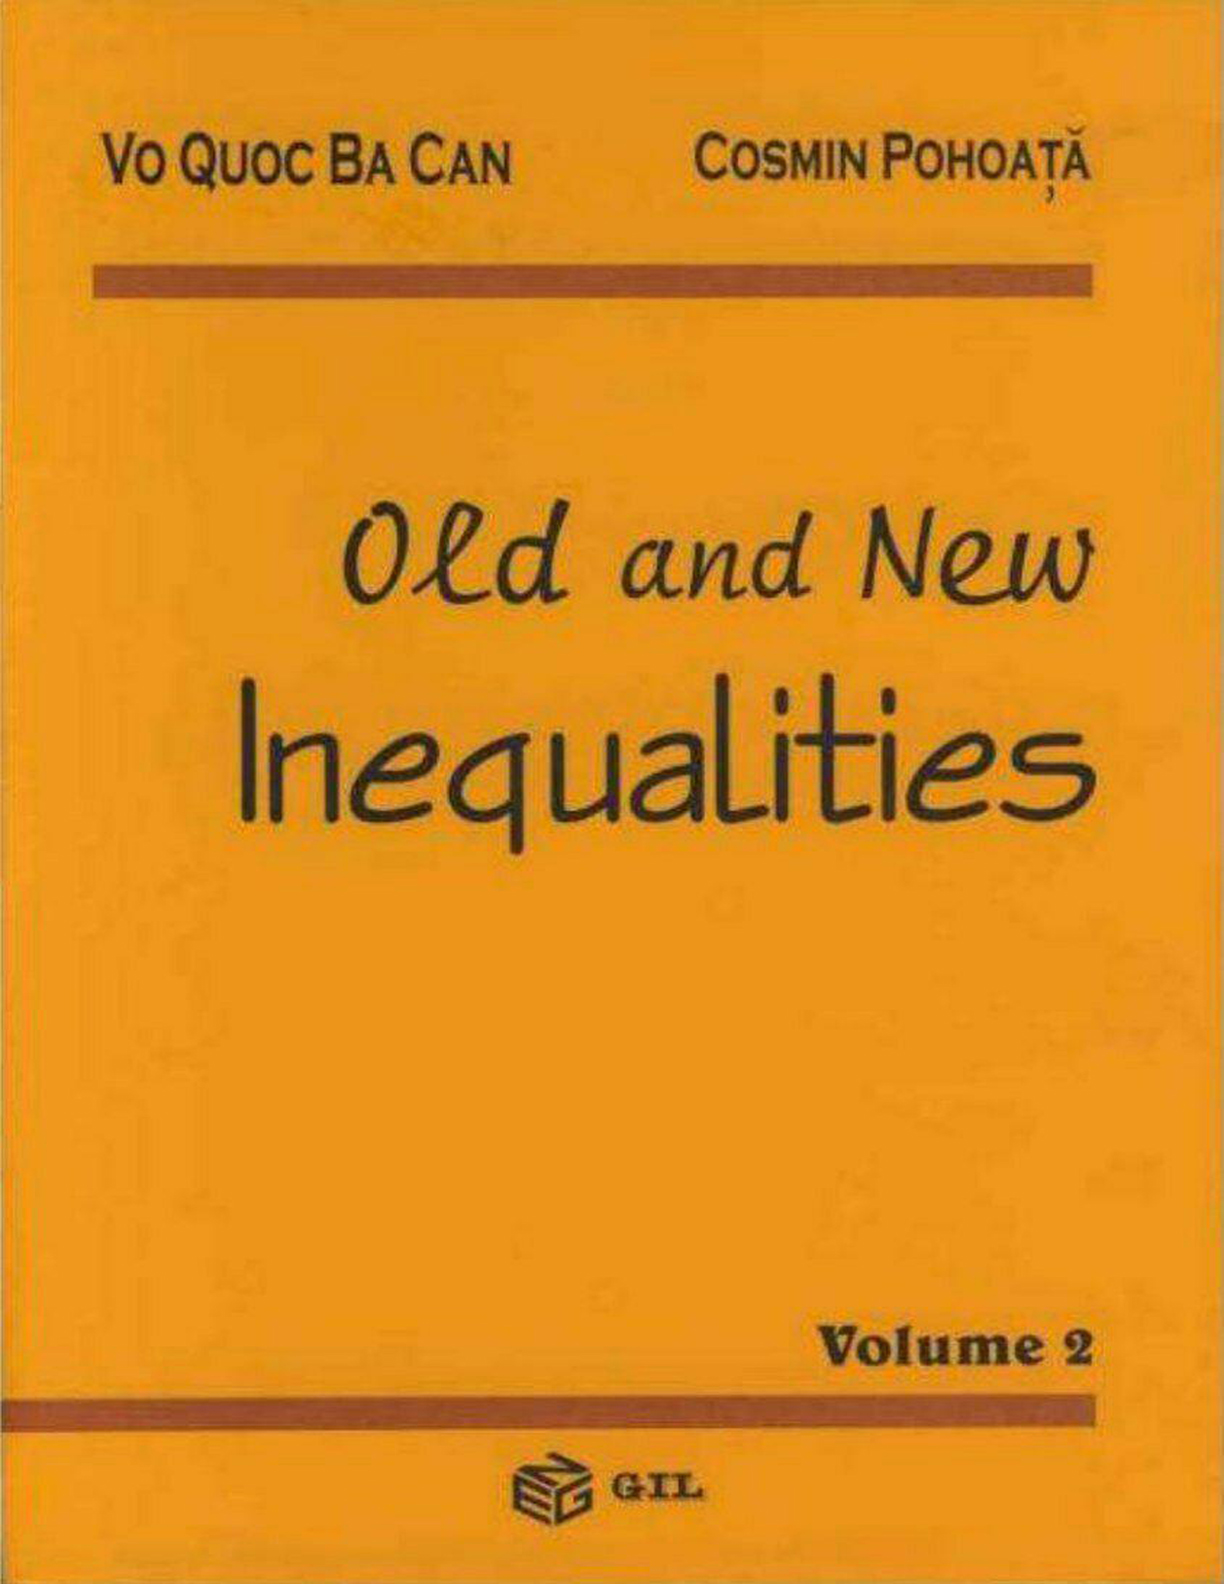
\includegraphics[width=\paperwidth]{1.jpg}}; % Background image
	\end{tikzpicture}};
\end{tikzpicture}
\vfill
\endgroup




\pagebreak



	
	
\thispagestyle{empty} 
	
\vspace*{4.5cm}
	
\begin{center}
\section*{Preface}
\end{center}
\begin{center}
\textit {”The last thing one knows when writing a book is what to put first.”}
\end{center}

\begin{flushright}
-{\itshape Blaise Pascal}
\end{flushright}
Mathematics has been called the science of tautology; that is to say, mathematicians have been accused of spending their time proving that things are equal to themselves. This statement is rather inaccurate on two counts. In the first place, mathematics, although the language of cience, is not a science. More likely it is a creative art, as G. H. Hardy liked to consider it. Secondly, the fundamental results of mathematics are often inequalities rather than equalities.\par
In the pages that follow, we present a large variety of problems involving such inequalities, questions that became famous in (mathematical) competitions or journals because of their beauty. The most important prerequisite for benefiting from this book is the desire to master the craft of discovery and proof. The formal requirements are quite modest. Anyone who knows basic inequalities such as the ones of \textbf {Cauchy-Schwarz}, \textbf{H\"{o}lder}, \textbf{Schur}, \textbf{Chebyshev} or \textbf{Bernoulli} is well prepared for almost everything to be found here. The student who is not that experienced will also be exposed in the first part to a wide combination of moderate and easy problems, ideas, techniques, and all the ingredients leading to a good preparation for mathematical contests. Some of the problems we chose to discuss are known, but we have included them here with new solutions which show the diversity of ideas pertaining to inequalities. Nevertheless, the book develops many results which are rarely seen, and even experienced readers are likely to find material that is challenging and informative.\par
To solve a problem is a very human undertaking, and more than a little mystery remains about how we best guide ourselves to the discovery of original solutions. Still, as George Pólya and the others have taught us, there are principles of problem solving. With practice and good coaching we can all improve our skills. Just like singers, actors, or pianists, we have a path toward a deeper mastery of our craft. 

	
\pagebreak
	
\thispagestyle{empty} 
	
\vspace*{5cm}
	
\begin{center}
\section*{About The Authors}
\end{center}

\textbf{Vo Quoc Ba Can} is a student at the ”Can Tho” University of Medicine and Pharmacy. As a high-school student, he participated in many national contests obtaining several prizes. Though at the moment he is not studying mathematics, his activity in Inequalities has proved to be quite wide lately. Some of his problems were published in specialized journals, but the biggest part of them became popular on the wordwide known MathLinks forum. On the same theme, he (co)authored several manuscripts, which were (unfortunately) published in Vietnamese.\par
\textbf{Cosmin Pohoat\v{a}} ¸ is in present a high-school student at the ”Tudor Vianu” High School in Bucharest, Romania. During his scholar activity he participated in many (mathematical or not) olympiads and contests. Recently, he was awarded with a Gold Medal at the Sharygin International Mathematical Olympiad, which took place in Dubna, Russia from July 29 to August 1, 2008. In the past few years, he had many important contributions in Euclidean Geometry, distinguishing himself in journals like Forum Geometricorum, Crux Mathematicorum or the American Mathematical Monthly. In Clark Kimberling’s Encyclopedia of Triangle Centers, a point appears under his name (X3333 - ”The Pohoata Point”). His main mathematical interests besides Euclidean Geometry are Graph Theory, Combinatorial Number Theory and, of course, Inequalities. Beyond mathematics, his activities include computer science, philosophy, music, football (soccer) and tennis.


	










\pagebreak

















\setcounter{page}{1}












	
\begin{center}
	\section*{Problems}
\end{center}


\begin{enumerate}
\item Prove that for all positive real numbers $a $, $b $ the following inequality holds $$\sqrt {2}\left (\sqrt {a (a+b)^3}+b\sqrt {a^2+b^2} \right )\leq 3\left (a^2+b^2 \right )$$
\begin{flushright}
\textbf{Irish MO, 2004}
\end{flushright}
\item Consider real numbers  $a $, $b $, $c $ contained in the interval  $\left [\frac {1}{2},1 \right ]$. Prove that $$2\leq \frac{a+b}{1+c}+ \frac{b+c}{1+a} +\frac{c+a}{1+b}\leq 3$$
\begin {flushright}
\textbf{Romanian MO, 2006}
\end{flushright}
\item Let $a$, $b$, $c$ be three positive real numbers contained in the interval  [0,1]. Prove that $$\frac {1}{1+ab}+\frac {1}{1+bc}+\frac {1}{1+ca}\leq \frac {5}{a+b+c}$$
\begin {flushright}
\textbf{Chendi Huang}
\end{flushright}
\item Let $x $, $y $, $z $ be positive reals with such that  $xyz=1$. Show that the following inequality holds $$\frac{1}{(1+x)^2+y^2+1}+\frac{1}{(1+y)^2+z^2+1}+\frac{1}{(1+z)^2+x^2+1} \leq  \frac{1}{2}$$ 
\begin {flushright}
\textbf{Cristinel Mortici, Math. Reflections}
\end{flushright}
\item Let $a$, $b$, $c$ be three positive real numbers satisfying $abc=8$. Prove that $$\frac {a-2}{a+1}+\frac {b-2}{b+1}+\frac {c-2}{c+1}\leq 0$$
\begin {flushright}
\textbf{Romaninan jBMO Team Preparation Tests, 2008}
\end{flushright}
\item Let $a$, $b$, $c$ be the side lengths of an acute-angled triangle. Prove that $$(a+b+c)(a^2+b^2+c^2)(a^3+b^3+c^3) \geq 4(a^6+b^6+c^6)$$
\begin {flushright}
\textbf{Vietnamese IMO Team Preparation Tests, 2000}
\end{flushright}
\item Let $a$, $b$, $c$ be positive real numbers such that $ab+bc+ca=1$. Prove that $$a\sqrt {b^2+c^2+bc} + b\sqrt {c^2+a^2+ca}+c\sqrt {a^2+b^2+ab}\geq \sqrt {3}$$
\begin {flushright}
\textbf{Jose Luis Diaz-Barrero, College Math. Journal}
\end{flushright}
\item Find the maximum value of $$(x^3+1)(y^3+1)$$ for all real numbers $x $, $y $, satisfying the condition that $x+y=1$
\begin {flushright}
\textbf{Romanian MO, 2006}
\end{flushright}
\pagebreak

\item Let $a$, $b$, $c$ be positive real numbers. Prove that $$\frac{a}{b}+ \frac{b}{c} + \frac{c}{a} \geq \frac{a+b}{b+c} +\frac{b+c}{a+b} +1$$
\begin {flushright}
\textbf{Bielorussian MO, 1998}
\end{flushright}
\item If $x $, $y $, $z $ are positive real numbers, prove that the following inequality holds $$(x+y+z)^2(xy+yz+zx)^2\leq 3 (y^2+yz+z^2)(z^2+zx+x^2)(x^2+xy+y^2)$$
\begin {flushright}
\textbf{Indian MO, 2007}
\end{flushright}
\item Let $a$, $b$, $c$ be positive real numbers such that $a+b+c \geq \displaystyle {\frac{1}{a}+ \frac{1}{b}+\frac{1}{c}}$. Prove that $$a+b+c \geq \frac{3}{a+b+c}+ \frac{2}{abc}$$
\begin {flushright}
\textbf{Peruvian IMO Team Selection Tests, 2007}
\end{flushright}
\item Let $a$, $b$, $c$ be positive real numbers such that $\displaystyle{\frac{1}{a+b+1} +\frac{1}{b+c+1} +\frac{1}{c+a+1} \geq 1}$. Prove that $$a+b+c \geq ab+bc+ca$$
\begin {flushright}
\textbf{Romanian jBMO Team Selection Tests, 2007}
\end{flushright}
\item Let $a$, $b$, $c$ be real numbers satisfying  $a$, $b $, $c \geq 1$ and $a+b+c =2abc $. Prove that $$\sqrt [3]{(a+b+c)^2} \geq \sqrt [3]{ab-1}+ \sqrt [3]{bc-1}+ \sqrt [3]{ca-1}$$
\begin {flushright}
\textbf{Bruno De Lima Holanda, Math. Reflections}
\end{flushright}
\item Let $a_1,\ a_2,\ \cdots, \ a_n $ be positive real numbers satisfying the condition that  $a_1+a_2+\cdots+a_n=1$. Prove that $$\sum \limits_{j=1}^n \frac{a_j}{1+a_1+\cdots + a_j}< \frac{1}{\sqrt {2}}$$
\begin {flushright}
\textbf{Romaninan IMO Team Preparation Tests, 2008}
\end{flushright}
\item Positive numbers $\alpha ,\ \beta,\ x_1,\ x_2,\ \cdots,\ x_n$ ($n\geq 1$) satisfy the condition  $x_1+x _2+\cdots + x_n=1$. Prove that $$\frac {x_1^3}{\alpha x_1+ \beta x_2} + \frac {x_2^3}{\alpha x_2+ \beta x_3} + \cdots + \frac {x_n^3}{\alpha x_n+ \beta x_1} \geq \frac {1}{n (\alpha + \beta )}$$
\begin {flushright}
\textbf{Moldavian IMO Team Selection Tests, 2002}
\end{flushright}
\item If three non negative real numbers $a $, $b $, $c $ satisfy the condition  $\displaystyle{\frac {1}{a^2+1}+\frac {1}{b^2+1}+\frac {1}{c^2+1}=2}$. Prove that  $$ab+bc+ca \leq \frac{3}{2}$$
\begin {flushright}
\textbf{Iranian MO, 2005}
\end{flushright}
\item Let $a$, $b$, $c$ be positive real numbers. Prove that  $$\frac {a^2}{b}+ \frac {b^2}{c}+ \frac {c^2}{a} \geq a+b+c+ \frac {4 (a-b)^2}{a+b+c}$$
\begin {flushright}
\textbf{Balkan MO, 2005}
\end{flushright}
\item If $x $, $y $, $z $ are positive numbers satisfying the condition  $xy+yz+zx=1$, show that  $$\frac {27}{4}(x+y)(y+z)(z+x)\geq \left (\sqrt {x+y}+\sqrt {y+z} + \sqrt {z+x} \right)^2\geq 6\sqrt {3}$$
\begin {flushright}
\textbf{Turkish IMO Team Selection Tests, 2006}
\end{flushright}
\item Let $a$, $b$, $c$ be positive real numbers. Prove that  $$\frac {a}{b}+\frac {b}{c}+\frac {c}{a} \geq 3+ \frac {(a-c)^2}{ab+bc+ca}$$
\begin {flushright}
\textbf {Vo Quoc Ba Can}
\end {flushright}
\item Let $a$, $b$, $c$ be non negative real numbers satisfying  $ab+bc+ca=3$. Prove that  $$\frac {1}{1+a^2 (b+c)}+\frac {1}{1+b^2 (c+a)}+\frac {1}{1+c^2 (a+b)}\leq \frac {3}{1+2abc}$$
\begin {flushright}
\textbf{Mathlinks Contest, 2008}
\end{flushright}
\item Let $a$, $b$, $c$ be positive real numbers such that $2a+b=1$. Prove that $$\frac{5a^3}{bc}+\frac{4b^3}{ca} +\frac{3c^3}{ab} \geq 4$$
\begin {flushright}
\textbf {Tran Van Luan}
\end {flushright}
\item \begin {enumerate}
      \item If $x $, $y $ and $z $ are three real numbers, all different from 1, such that  $xyz=1$, prove that  $$\frac {x^2}{(x-1)^2}+ \frac{y^2}{(y-1)^2}+\frac {z^2}{(z-1)^2}\geq 1$$
      \item Prove that equality is achieved for infinitely many triples of rational numbers $x $, $y $ and $z $.
      \end {enumerate}
\begin {flushright}
\textbf{IMO, 2008}
\end{flushright}
\item Let $a$, $b$, $c$ be positive real numbers. Prove that $$\frac {a}{b(b+c)^2}+\frac {b}{c (c+a)^2}+\frac {c}{a (a+b)^2} \geq \frac {9}{4 (ab+bc+ca)}$$
\begin {flushright}
\textbf{Ho Phu Thai, Math. Reflections}
\end{flushright}
\item Let $a$, $b$, $c$ be non negative real numbers such that $a+b+c=1$. Prove that $$\sqrt {a+\frac {(b-c)^2}{4}}+\sqrt {b}+\sqrt {c}\leq \sqrt {3}$$
\begin {flushright}
\textbf{Chinese Girls MO, 2008}
\end{flushright}
\item Let $a$, $b$, $c$ be the side lengths of a triangle. Prove that $$\sum \limits_{cyc} \frac {a^3}{a^3+(b+c)^3}+1\geq 2\sum \limits_{cyc}\frac {a^2}{a^2+(b+c)^2}$$
\begin {flushright}
\textbf{Pham Quang Vu}
\end{flushright}
\pagebreak

\item Prove that for any real numbers $a $, $b $, $c $ the following inequality holds  $$(a+b-c)^2(b+c-a)^2(c+a-b)^2\geq (a^2+b^2-c^2)(b^2+c^2-a^2)  ( c^2+a^2-b^2)$$
\begin {flushright}
\textbf{Japanese MO, 2001}
\end{flushright}
\item Let $a$, $b$, $c$ be the side lengths of a triangle. Prove that $$(a+b)(b+c)(c+a)+(a+b-c)(b+c-a)(c+a-b)\geq 9abc $$
\begin {flushright}
\textbf{Virgil Nicula and Cosmin Pohoata, Math. Reflections}
\end{flushright}
\item Let $a$, $b$, $c$ be positive real numbers. Prove that $$\left (\frac {1}{a}+\frac {1}{b}+\frac {1}{c} \right )\left (\frac {1}{a+1}+\frac {1}{b+1}+\frac {1}{c+1} \right )\geq \frac{9}{abc+1}$$
\begin {flushright}
\textbf{Walther Janous}
\end{flushright}
\item Let $a$, $b$, $c$ be positive real numbers contained in the interval [0,1]. Prove that $$\frac{2a}{1+bc}+\frac{2b}{1+ca}+\frac{2c}{1+ab}+abc\leq 4$$
\begin {flushright}
\textbf{Adapted after Polish MO, 2005}
\end{flushright}
\item Let $a$, $b$, $c$ be non negative real numbers satisfying  $Max\{b+c-a,\ c+a-b,\ a+b-c \}\leq 1$. Prove that  $$a^2+b^2+c^2\leq 1+2abc$$
\begin {flushright}
\textbf{Chendi Huang}
\end{flushright}
\item If $x $, $y $, $z $ are real numbers satisfying  $xyz=-1$, prove that $$x^4+y^4+z^4+3 (x+y+z)\geq \frac {y^2+z^2}{x}+\frac {z^2+x^2}{y}+\frac {x^2+y^2}{z}$$
\begin {flushright}
\textbf{Iranian MO, 2005}
\end{flushright}
\item Let $a $, $b $,$c $, $d $ be positive real numbers satisfying the condition  $a+b+c+d=abc+bcd+cda+dab $. Prove that  $$a+b+c+d+\frac {2a}{a+1}+\frac {2b}{b+1}+\frac {2c}{c+1}+\frac {2d}{d+1}\geq 8$$
\begin {flushright}
\textbf{Vo Quoc Ba Can}
\end{flushright}
\item Let $a$, $b$, $c$ be non negative real numbers. Prove that $$\frac {a^2+2bc}{b^2+c^2}+\frac {b^2+2ca}{c^2+a^2}+\frac {c^2+2ab}{a^2+b^2}\geq 3$$
\begin {flushright}
\textbf{Russian MO, 1999}
\end{flushright}
\pagebreak 

\item Let $a$, $b$, $c$ be positive real numbers. Prove that $$\frac {ab}{c (c+a)}+\frac {bc}{a (a+b)}+\frac {ca}{b (b+c)}\geq \frac {a}{c+a}+\frac {b}{a+b}+\frac {c}{b+c}$$
\begin {flushright}
\textbf{Moldavian MO, 1999}
\end{flushright}
\item Let $a$, $b$, $c$ be positive real numbers such that $ab+bc+ca\geq 3$. prove that $$\frac {a}{\sqrt {a+b}}+\frac {b}{\sqrt {b+c}}+\frac {c}{\sqrt {c+a}}\geq \frac {3}{\sqrt {2}}$$
\begin {flushright}
\textbf{Pham Huu Duc, Math. Reflections}
\end{flushright}
\item Let $x$, $y$, $z$, $t $ be positive real numbers such that $\displaystyle{\frac {1}{x+1}+\frac {1}{y+1}+\frac {1}{z+1}+\frac {1}{t+1}}=1$. Prove that $$min\left \{\frac {1}{x}+\frac {1}{y}+\frac {1}{z};\ \frac {1}{y}+\frac {1}{z}+\frac {1}{t};\ \frac {1}{z}+\frac {1}{t}+\frac {1}{x};\    \frac {1}{t}+\frac {1}{x}+\frac {1}{y}\right \}\leq 1 $$

$$\leq max\left \{\frac {1}{x}+\frac {1}{y}+\frac {1}{z};\ \frac {1}{y}+\frac {1}{z}+\frac {1}{t};\ \frac {1}{z}+\frac {1}{t}+\frac {1}{x};\    \frac {1}{t}+\frac {1}{x}+\frac {1}{y}\right \}$$
\begin {flushright}
\textbf{Pham Van Thuan}
\end{flushright}
\item Let $a_1,\ a_2,\ \cdots ,\ a_n $ be positive real numbers. Prove that $$\prod \limits_{k=1}^n \left (\sum \limits_{j=1}^na_j^{T_k} \right )\geq  \left (\sum \limits_{k=1}^na_n^{\frac {T_{n+1}}{3}} \right )^n$$ where $T_k = \displaystyle{\frac {k (k+1)}{2}}$ is the $k-$th triangular number.
\begin {flushright}
\textbf{Jose Luis Diaz-Barrero, Math. Reflections}
\end{flushright}
\item Let $a$, $b$, $c$, $d $ be positive numbers. Prove that $$3 (a^2-ab+b^2)(c^2-cd+d^2)\geq (a^2c^2-abcd+b^2d^2)$$
\begin {flushright}
\textbf{Titu Andreescu, Math. Reflections}
\end{flushright}
\item Let $a$, $b$, $c$, $d $ be real numbers such that $a+b+c=1$. Prove that $$\frac {a}{a^2+1}+\frac {b}{b^2+1}+\frac{c}{c^2+1}\leq \frac{9}{10}$$
\begin {flushright}
\textbf{Polish MO, 1997}
\end{flushright}
\item Let $n $ be a positive integer, and let $x $ and $y $ be positive real numbers such that $x^n+y^n=1$. Prove that $$\left (\sum \limits_{k=1}^n \frac {1+x^{2k}}{1+x^{4k}}\right )\left (\sum \limits_{k=1}^n \frac {1+y^{2k}}{1+y^{4k}} \right )< \frac {1}{(1-x)(1-y)}$$
\begin {flushright}
\textbf{IMO Shortlist, 2007, proposed by Estonia}
\end{flushright}
\pagebreak 

\item Let $a$, $b$, $c$ be positive real numbers such that $a+b+c+1=4abc$. Prove that $$\frac{1}{a}+\frac{1}{b}+\frac{1}{c} \geq 3 \geq \frac{1}{\sqrt {ab}}+\frac{1}{\sqrt {bc}}+\frac{1}{\sqrt{ca}}$$
\begin {flushright}
\textbf{Daniel Campos Salas, Math. Reflections}
\end{flushright}
\item Let $a$, $b$, $c$ be nonnegative real numbers such that $a+b+c=3$ Set $x=\sqrt{a^2-a+1}$, $y=\sqrt{b^2-b+1}$ and $z=\sqrt{c^2-c+1}$. Prove that  $$xy+yz+zx\geq 3\ \text{and} \ x+y+z\leq 2+\sqrt{7}$$
\begin {flushright}
\textbf{Adapted after the Vietnamese MO, 2007}
\end{flushright}
\item Let $n\geq 2$ be a given integer. Determine 
\begin {enumerate}
\item The largest real $c_n $ such that  $$\frac {1}{1+a_1}+\frac {1}{1+a_2}+\cdots +\frac {1}{1+a_n} \geq c_n$$ holds for any positive numbers $a_1,\ a_2,\ \cdots,\ a_n$ with $a_1a_2\cdots a_n =1$
\item The largest real $d_n$ such that $$\frac {1}{1+2a_1}+\frac {1}{1+2a_2}+\cdots +\frac {1}{1+2a_n} \geq d_n$$ holds for any positive numbers $a_1,\ a_2,\ \cdots,\ a_n$ with $a_1a_2\cdots a_n =1$
\end {enumerate}
\begin {flushright}
\textbf{Italian MO, 2007}
\end{flushright}
\item Let $a$, $b$, $c$ be positive real numbers. Prove that $$\frac {bc}{a^2+bc}+\frac {ca}{ab^2+ca}+\frac {ab}{c^2+ab}\leq \frac {a}{b+c}+\frac {b}{c+a}+\frac {c}{a+b}$$
\begin {flushright}
\textbf{Pham Huu Duc, Math. Reflections}
\end{flushright}
\item Real numbers $a_1, a_2, \cdots, a_n$ are given. For each $i $ $(1\leq i \leq n)$ define $d_i=max\{a_j\ |\ 1\leq j \leq i \} -min\{a_j\ |\ i\leq j \leq n \}$ and let $d = max \{d_i\ |\ 1\leq i \leq n \}$
\begin {enumerate}
\item Prove that for any real numbers $x_1\leq x_2\leq \cdots \leq x_n$, we have $$max\{|x_i-a_i|\ |\ 1\leq i\leq n \}\geq \frac {d}{2}$$
\item Show that there are real numbers $x_1\leq x_2\leq \cdots \leq x_n$ such that we have equality in (a)
\end {enumerate}
\begin {flushright}
\textbf{IMO, 2007, Proposed by New Zealand}
\end{flushright}
\item Let $a$, $b$, $c$ be nonzero positive numbers. Prove that $$\sqrt{\frac{a^2}{4a^2+ab+4b^2}}+\sqrt{\frac{b^2}{4b^2+bc+4c^2}}+\sqrt{\frac{c^2}{4a^2+ca+4a^2}}\leq 1$$
\begin {flushright}
\textbf{Zhao Bin, Math. Reflections}
\end{flushright}
\item Let $a$, $b$, $c$ be positive numbers such  that $4abc = a+b+c+1$. Prove that $$\frac {b^2+c^2}{a}+\frac {c^2+a^2}{b}+\frac {a^2+b^2}{c}\geq 2 (ab+bc+ca)$$
\begin {flushright}
\textbf{Andrei Ciupan, Math. Reflections}
\end{flushright}
\item Let $a$, $b$, $c$ be positive numbers. Prove that $$\frac {a^3}{(a+b)^3}+\frac {b^3}{(b+c)^3}+\frac {c^3}{(c+a)^3}\geq \frac {3}{8}$$
\begin {flushright}
\textbf{Vietnamese IMO Team Selection Tests, 2005}
\end{flushright}
\item Let $a$, $b$, $c$, $x $, $y $, $z $ be positive real numbers. Prove that $$(a^2+x^2)(b^2+y^2)(c^2+z^2)\geq (ayz+bzx+cxy-xyz)^2$$
\begin {flushright}
\textbf{Titu Andreescu, Math. Reflections}
\end{flushright}
\item Let $x $, $y $, $z $ be positive real numbers. Prove that $$\frac {\sqrt {y+z}}{x}+\frac {\sqrt {z+x}}{y}+\frac {\sqrt {x+y}}{z} \geq \frac {4 (x+y+z)}{\sqrt {(x+y)(y+z)(z+x)}}$$
\begin {flushright}
\textbf{Darij Grinberg}
\end{flushright}
\item Let $a$, $b$ ,$c$ be nonnegative real numbers such that $abc = 4$ and $a, b, c > 1$. Prove that $$(a-1)(b-1)(c-1)(\frac{a+b+c}{3}-1)\leq \left(\sqrt[3]{4}-1\right)^4$$
\begin {flushright}
\textbf{Marian Tetiva, Math. Reflections}
\end{flushright}
\item Let $a$ ,$b$, $c$ be positive real numbers satisfying $abc = 1$. Prove that $$\frac{1}{b(a+b)}+\frac{1}{c(b+c)}+\frac{1}{a(c+a)}\geq \frac{3}{2}$$
\begin {flushright}
\textbf{Kazakhstan, Zhautykov Olympiad, 2008}
\end{flushright}
\item Prove that for all positive real numbers $a$, $b$, $c$ the following inequality holds: $$\frac{1}{a+b+c}\left(\frac{1}{b+c}+\frac{1}{c+a}+\frac{1}{a+b}\right)\geq \frac{1}{ab+bc+ca}+\frac{1}{2(a^2+b^2+c^2)}$$
\begin {flushright}
\textbf{Pham Huu Duc, Math. Reflections}
\end{flushright}
\item Let $a$, $b$, $c$ be the sidelengths of a triangle. Prove that $$\frac{\sqrt{b+c-a}}{\sqrt{b}+\sqrt{c}-\sqrt{a}}+\frac{\sqrt{c+a-b}}{\sqrt{c}+\sqrt{a}-\sqrt{b}}+\frac{\sqrt{a+b-c}}{\sqrt{a}+\sqrt{b}-\sqrt{c}}\leq 3$$
\begin {flushright}
\textbf{IMO Shortlist, 2006, Proposed by South Korea}
\end{flushright}
\item Let $a$, $b$, $c$ be the sidelengths of a triangle with perimeter 1. Prove that $$1<\frac{b}{\sqrt{a+b^2}}+\frac{c}{\sqrt{b+c^2}}+\frac{a}{\sqrt{c+a^2}}<2$$
\begin {flushright}
\textbf{Vo Quoc Ba Can}
\end{flushright}
\item Prove that for any positive real numbers $a$, $b$ and $c$, we have that $$\sqrt{\frac{b+c}{a}}+\sqrt{\frac{c+a}{b}}+\sqrt{\frac{a+b}{c}}\geq \sqrt{6\frac{a+b+c}{\sqrt[3]{abc}}}$$
\begin {flushright}
\textbf{Pham Huu Duc, Math. Reflections}
\end{flushright}
\item Let $a$ ,$b$, $c$ be positive real numbers. Prove that $$\frac{a}{\sqrt{ab+b^2}}+\frac{b}{\sqrt{bc+c^2}}+\frac{c}{\sqrt{ca+a^2}}\geq \frac{3}{\sqrt{2}}$$
\begin {flushright}
\textbf{Cosmin Pohoata and Michael Rozenberg}
\end{flushright}
\item Let $a_1 \leq a_2 \leq \cdots \leq a_n$ be positive real numbers such that $\displaystyle{\frac{a_1^2+a_2^2+\cdots +a_n^2}{n}}=1,$\\
$\displaystyle{\frac{a_1+a_2+\cdots +a_n}{n}}=m$ where $1 \geq m > 0$. Prove that for all $i$ satisfying $a_i \leq m$, we have $$n-i\geq n(m-a_i)^2$$
\begin {flushright}
\textbf{Iranian IMO Team Selection Test, 2005}
\end{flushright}
\item Let $x$ ,$y$, $z$ be positive real numbers. Prove that $$\frac{3\sqrt{3}}{2}\leq \sqrt{x+y+z}\left(\frac{\sqrt{x}}{y+z}+\frac{\sqrt{y}}{z+x}+\frac{\sqrt{z}}{x+y}\right)$$
\begin {flushright}
\textbf{Byron Schmuland, Math. Reflections}
\end{flushright}
\item Let $a$ ,$b$, $c$ be positive real numbers. Prove that $$\frac{a}{\sqrt{a^2+2bc}}+\frac{b}{\sqrt{b^2+2ca}}+\frac{c}{\sqrt{c^2+2ab}}\leq \frac{a+b+c}{\sqrt{ab+bc+ca}}$$
\begin {flushright}
\textbf{Ho Phu Thai, Math. Reflections}
\end{flushright}
\item Let $a$ ,$b$, $c$ be distinct positive real numbers. Prove the following inequality $$\frac{a^2b+a^2c+b^2a+b^2c+c^2a+c^2b-6abc}{a^2+b^2+c^2-ab-bc-ca}\geq \frac{16abc}{(a+b+c)^2}$$
\begin {flushright}
\textbf{Iurie Boreico and Ivan Borsenco, Math. Reflections}
\end{flushright}
\item Let $a$ ,$b$, $c$ be nonzero positive real numbers. Prove that $$\frac{a^3+abc}{b+c}+\frac{b^3+abc}{c+a}+\frac{c^3+abc}{a+b}\geq \frac{a(b^3+c^3)}{a^2+bc}+\frac{b(c^3+a^3)}{b^2+ca}+\frac{c(a^3+b^3)}{c^2+ab}$$
\begin {flushright}
\textbf{Pham Huu Duc and Cosmin Pohoata}
\end{flushright}
\item Let $a$, $b$, $c$, $d$ be real numbers with sum 0. Prove that $$(ab+ac+ad+bc+bd+cd)^2+12\geq 6(abc+abd+acd+bcd)$$
\begin {flushright}
\textbf{Kazakhstan, Zhautykov Olympiad, 2006}
\end{flushright}

\pagebreak

\item Let $a$ ,$b$, $c$ be positive real numbers satisfying $a+b+c=1$. Prove that $$\left(\frac{1}{a}-2\right)^2+\left(\frac{1}{b}-2\right)^2+\left(\frac{1}{c}-2\right)^2 \geq \frac{8(a^2+b^2+c^2)^2}{(1-a)(1-b)(1-c)} $$
\begin {flushright}
\textbf{Vo Quoc Ba Can, Math. and Youth magazine}
\end{flushright}
\item Let $x_1,x_2,\cdots ,x_n$ be real numbers from the interval $[0,1]$ satisfying $x_1x_2\cdots x_n =\\ (1-x_1)^2 (1-x_2)^2\cdots (1-x_n)^2$. Find the maximum value of $x_1x_2\cdots x_n$
\begin {flushright}
\textbf{Chendi Huang}
\end{flushright}
\item Let $a$, $b$, $c$ be three positive real numbers with sum 3. Prove that $$\frac{1}{a^2}+\frac{1}{b^2}+\frac{1}{c^2}\geq a^2+b^2+c^2$$
\begin {flushright}
\textbf{Romanian IMO Team Selection Tests, 2006}
\end{flushright}
\item Let $a$ ,$b$, $c$ be positive real numbers satisfying $a+b+c=1$. Prove that $$\frac{a}{2b+1}+\frac{b}{2c+1}+\frac{c}{2a+1}\leq \frac{1}{abc}$$
\begin{flushright}
\textbf{Vo Quoc Ba Can}
\end{flushright}
\item For any three positive numbers $a$, $b$, $c$, prove the inequality $$(1+abc)\left(\frac{1}{a(1+b)}+\frac{1}{b(1+c)}+\frac{1}{c(1+a)}\right)\geq 3$$
\begin{flushright}
\textbf{BMO, 2006}
\end{flushright}
\item Let $a$, $b$, $c$, $d$ be real numbers such that $a^2+b^2+c^2+d^2=1$. Prove that $$\frac{1}{1-ab}+\frac{1}{1-bc}+\frac{1}{1-ca}+\frac{1}{1-da}\leq \frac{16}{3}$$
\begin{flushright}
\textbf{Vo Quoc Ba Can}
\end{flushright}
\item  Let $x_1,x_2,\cdots ,x_n$ be positive real numbers such that $x_1+x_2+\cdots +x_n=1$. Prove that $$\left(\sum \limits_{i=1}^n\sqrt{x_i}\right)\left(\sum \limits_{i=1}^n \frac{1}{1+\sqrt{x_i}}\right)\leq \frac{n^2}{\sqrt{n+1}}$$
\begin{flushright}
\textbf{Chinese TST, 2006}
\end{flushright}
\item Let $a$ ,$b$, $c$ be positive real numbers. Prove that $$\frac{a^4+b^4+c^4}{ab+bc+ca}+\frac{3abc}{a+b+c}\geq \frac{2}{3}\left(a^2+b^2+c^2\right)$$
\begin{flushright}
	\textbf{Vo Quoc Ba Can, Cosmin Pohoata}
\end{flushright}
\item Let $a$ ,$b$, $c$ be nonnegative real numbers, from which at least two are nonzero. Prove that $$\sqrt[3]{\frac{a^2+bc}{b^+c^2}}+\sqrt[3]{\frac{b^2+ca}{c^+a^2}}+\sqrt[3]{\frac{c^2+ab}{a^+b^2}}\geq\frac{\sqrt[3]{9abc}}{a+b+c}$$
\begin{flushright}
	\textbf{Pham Huu Duc, Math. Reflections}
\end{flushright}
\item Let $a_1,a_2,\cdots ,a_{100}$ be nonnegative real numbers such that $a_1^2+a_2^2+\cdots+a_{100}^2=1$. Prove that$$a_1^2a_2+a_2^2a_3+\cdots+a_{100}^2a_1<\frac{12}{25}$$
\begin{flushright}
	\textbf{IMO Shortlist, 2007, Proposed by Poland}
\end{flushright}
\item Let $a$ ,$b$, $c$ be nonnegative real numbers, no two of which are zero. Prove that $$\frac{ab+ac+4bc}{b^2+c^2}+\frac{bc+ba+4ca}{c^2+a^2}+\frac{ca+cb+4ab}{a^2+b^2}\geq 4$$
\begin{flushright}
	\textbf{Vasile Cirtoaje}
\end{flushright}
\item Let $a$ ,$b$, $c$ be positive real numbers. Prove that $$\frac{a+b^2+c^3}{ab+c^2}+\frac{b+c^2+a^3}{bc+a^2}+\frac{c+a^2+b^3}{ca+b^2}\geq \frac{9}{2}$$
\begin{flushright}
	\textbf{Vo Quoc Ba Can}
\end{flushright}
\item Let $a$ ,$b$ and $c$ be positive real numbers satisfying $a+b+c=2$. Prove that $$\frac{1}{2}+\sum \limits_{cyc}\frac{a}{b+c}\leq \frac{a^2+bc}{b+c}+\frac{b^2+ca}{c+a}+\frac{c^2+ab}{a+b}\leq \frac{1}{2}+\sum \limits_{cyc} \frac{a^2}{b^2+c^2}$$
\begin{flushright}
	\textbf{Cosmin Pohoata}
\end{flushright}
\item Real number $a_i$, $b_i$ ($1\leq i\leq n$) satisfy $\sum \limits_{i=1}^n a_i^2=\sum \limits_{i=1}^n b_i^2=1$ and $\sum \limits_{i=1}^n a_ib_i=0$. Prove that $$\left(\sum \limits_{i=1}^n a_i\right)^2+\left(\sum \limits_{i=1}^n b_i\right)^2\leq n$$
\begin{flushright}
	\textbf{BMO Shortlist, 2007, Proposed by Romania}
\end{flushright}
\item Let $a$ ,$b$ and $c$ be positive real numbers satisfying $a+b+c=1$. Prove that$$\frac{ab}{\sqrt{ab+bc}}+\frac{bc}{\sqrt{bc+ca}}+\frac{ca}{\sqrt{ca+ab}}\geq \frac{\sqrt{2}}{2}$$
\begin{flushright}
	\textbf{Chinese MO, 2006}
\end{flushright}
\item Let $a$ ,$b$ and $c$ be nonnegative real numbers satisfying $a^2+b^2+c^2=1$. Prove that$$1\leq \frac{a}{1+bc}+\frac{b}{1+ca}+\frac{c}{1+ab}\leq \sqrt{2}$$
\begin{flushright}
	\textbf{Faruk Zejnulahi, Crux Math.}
\end{flushright}

\pagebreak

\item Let $a$ ,$b$ and $c$ be positive real numbers such that $a\leq b\leq c$ and $abc=1$. Prove that$$a+b^2+c^3 \geq \frac{1}{a}+\frac{1}{b^2}+\frac{1}{c^3}$$
\begin{flushright}
	\textbf{Vo Quoc Ba Can}
\end{flushright}
\item Given $k+1$ positive real numbers $x_0,x_1,x_2,\cdots ,x_k$ and a positive integer $n$. Show that $$\left(x_{\sigma_1}+x_{\sigma_2}+\cdots+x_{\sigma_k}\right)^{-n}\leq k^{-n}\sum \limits_{i=0}^kx_i^{-n}$$where the sum on the left is taken of the $k + 1$ distinct $k-$element subsets of $\{x_0,x_1,\cdots,x_k\}$
\begin{flushright}
	\textbf{Emre Alkan, Amer. Math. Monthly}
\end{flushright}
\item Let $a$, $b$, $c$ be nonnegative real numbers, such that at least two are nonzero and which satisfy the condition $a + b + c = 1$. Prove that$$\frac{a}{\sqrt{a+2b}}+\frac{b}{\sqrt{b+2c}}+\frac{c}{\sqrt{c+2a}}\leq \frac{\sqrt[4]{27}\left(\sqrt{3}-1\right)}{\sqrt{2}}$$
\begin{flushright}
	\textbf{Vo Quoc Ba Can, Pham Kim Hung}
\end{flushright}
\item For Real numbers $x_i>1$, $1\leq i\leq n$, $n\geq 2$ such that $$\frac{x_i^2}{x_i-1}\geq S=\sum \limits_{j=1}^n x_j,\ \operatorname{for\  all}\ i=1,2,\cdots,n$$find with proof $sup\ S$
\begin{flushright}
	\textbf{Romanian IMO Team Preparation Tests, 2008}
\end{flushright}
\item Let $a$ ,$b$, $c$, $d$ be positive real numbers such that $a+b+c+d=abc+bcd+cda+dab$. Prove that $$\left(\sqrt{a^2+1}+\sqrt{b^2+1}\right)^2+\left(\sqrt{c^2+1}+\sqrt{d^2+1}\right)^2\leq (a+b+c+d)^2$$
\begin{flushright}
	\textbf{Vo Quoc Ba Can}
\end{flushright}
\item Let $a$, $b$, $c$ be the sidelengths of a triangle. Prove that $$a^2\left(\frac{b}{c}-1\right)+b^2\left(\frac{c}{a}-1\right)+c^2\left(\frac{a}{b}-1\right)\geq 0$$
\begin{flushright}
	\textbf{Moldavian IMO Team Selection Test, 2006}
\end{flushright}
\item Let $x$ ,$y$, $z$ be positive real numbers such that  $x^2+y^2+z^2\geq 3$. Prove that$$\frac{x^5-x^2}{x^5+y^2+z^2}+\frac{y^5-y^2}{y^5+z^2+x^2}+\frac{z^5-z^2}{z^5+x^2+y^2}\geq 0$$
\begin{flushright}
	\textbf{Vasile Cirtoaje}
\end{flushright}
\item Let $a$, $b$, $c$ be the sidelengths of a triangle. Prove that$$\frac{a}{b}+\frac{b}{c}+\frac{c}{a}\geq 2\left(\frac{a+b}{b+c}+\frac{b+c}{c+a}+\frac{c+a}{a+b}\right)$$
\begin{flushright}
	\textbf{Vo Quoc Ba Can}
\end{flushright}
\item Let $x$ ,$y$, $z$ be positive real numbers. Prove that $$\left(\frac{x+y}{z}+\frac{y+z}{x}+\frac{z+x}{y}\right)-4\left(\frac{x}{y+z}+\frac{y}{z+x}+\frac{z}{x+y}\right)\geq 1-\frac{8xyz}{(x+y)(y+z)(z+x)}$$
\begin{flushright}
	\textbf{Cezar Lupu and Cosmin Pohoata, La Gaceta de la RSME}
\end{flushright}
\item Let $x$ ,$y$, $z$ be real numbers satisfying $a^2+b^2+c^2=9$. Prove that $$3\times min\{a,b,c\}\leq 1+abc$$
\begin{flushright}
	\textbf{Virgil Nicula, Crux Mathematicorum}
\end{flushright}
\item Let $x_1, x_2,\cdots , x_{3n}$ be positive real numbers. Prove that$$2^n\prod \limits_{k=1}^{3n}\frac{1+x_k^2}{1+x_k}\geq \left(1+\prod \limits_{k=1}^{3n} x_k^{\frac{1}{n}}\right)^n$$
\begin{flushright}
	\textbf{Mihaly Bencze, Math. Magazine}
\end{flushright}
\item Given an integer $n \geq 2$, find the largest constant $C(n)$ for which the inequality$$\sum \limits_{i=1}^nx_i\geq C(n)\sum \limits_{1\leq j< i\leq n}2x_ix_j+\sqrt{x_ix_j}$$holds for all real numbers $x_i \in(0, 1)$ satisfying $(1 - x_i)(1 - x_j) \leq \frac{1}{4}$ for $1 \leq j < i \leq n$
\begin{flushright}
	\textbf{Bulgarian IMO Team Selection Tests, 2007}
\end{flushright}
\item Let $a$, $b$, $c$ be nonnegative real numbers, from which at least two are nonzero and satisfying the condition $ab + bc + ca = 1$. Prove that $$\sqrt{a^3 + a} + \sqrt{b^3 + b} + \sqrt{c^3 + c} \geq 2\sqrt{a + b + c}$$
\begin{flushright}
	\textbf{Iran TST, 2008}
\end{flushright}
\item Let $a$, $b$, $c$ , $d$ be nonnegative real numbers such that $a + b + c + d = 3$. Prove that $$ab(a + 2b + 3c) + bc(b + 2c + 3d) + cd(c + 2d + 3a) + da(d + 2a + 3b) \leq 6\sqrt{3}$$
\begin{flushright}
	\textbf{Pham Kim Hung}
\end{flushright}
\item For $n \in \mathbb{N}$, $n \geq 2$, determine $$max\prod \limits_{i=1}^n\left(1-x_i\right),\ \operatorname{for}\ x_i \in \mathbb{R}_+,\ 1\leq i\leq n,\ \sum \limits_{i=1}^nx_i^2=1$$
\begin{flushright}
	\textbf{Romanian IMO Team Selection Tests, 2007}
\end{flushright}

\pagebreak

\item For integers $n \geq 2$ and real $s > 0$, show that$$\left(\prod \limits_{i=0}^n(s+i)\right)\left(\prod \limits_{j=0}^n\frac{1}{s+j}\right)<(n+1)\prod \limits_{k=1}^n\left(s+k-\frac{1}{2}\right)$$
\begin{flushright}
	\textbf{Robert E. Shafer, Amer. Math. Monthly}
\end{flushright}
\item Let $a$, $b$, $c$ be real numbers contained in the interval $\left[0, \frac{3}{5}\right]$ and also satisfying the condition $a + b + c = 1$.  Determine the maximum value that the following expression can reach: $$P(a,b,c)=a^3+b^3+c^3+\frac{3}{4}abc$$
\begin{flushright}
	\textbf{Vo Quoc Ba Can, After Chinese Northern MO, 2007}
\end{flushright}
\item Let $a$, $b$, $c$, $d$ be positive real numbers such that $a \geq b \geq c \geq d$ and $abcd=1$. Prove that $$\frac{1}{1+a^3}+\frac{1}{1+b^3}+\frac{1}{1+c^3}\geq \frac{3}{1+abc}$$
\begin{flushright}
	\textbf{MathLinks Contest, 2008}
\end{flushright}
\item Let $a$, $b$, $c$ be nonnegative real numbers, from which at least are nonzero. Prove that $$\frac{a^2(b+c)^2}{b^2+c^2}+\frac{b^2(c+a)^2}{c^2+a^2}+\frac{c^2(a+b)^2}{a^2+b^2}\geq 2(ab+bc+ca)$$
\begin{flushright}
	\textbf{Vo Quoc Ba Can, Cosmin Pohoata}
\end{flushright}
\item Let $a$, $b$, $c$ be nonnegative real numbers, from which at least two are nonzero. Prove that$$\frac{(a+b+c)^2}{ab+bc+ca}\geq \frac{a(b+c)}{a^2+bc}+\frac{b(c+a)}{b^2+ca}+\frac{c(a+b)}{c^2+ab}\geq\frac{(a+b+c)^2}{a^2+b^2+c^2}$$
\begin{flushright}
	\textbf{Tran Quoc Anh}
\end{flushright}
\item Let $a$, $b$, $c$ be positive real numbers. Prove that$$\frac{a^2-bc}{4a^2+4b^2+c^2}+\frac{b^2-ca}{4b^2+4c^2+a^2}+\frac{c^2-ab}{4c^2+4a^2+b^2}\geq 0$$
\begin{flushright}
	\textbf{Vasile Cirtoaje, Math. Reflections}
\end{flushright}
\item Let $a$, $b$, $c$ be nonnegative real numbers, from which at least two are nonzero. Prove that $$\frac{a(b+c)}{b^2+c^2}+\frac{b(c+a)}{c^2+a^2}+\frac{c(a+b)}{a^2+b^2}\geq \frac{a(b+c)}{a^2+bc}+\frac{b(c+a)}{b^2+ca}+\frac{c(a+b)}{c^2+ab}$$
\begin{flushright}
	\textbf{Vo Quoc Ba Can, Cosmin Pohoata}
\end{flushright}
\item Let $n$ be a positive integer. Find the minimum value of$$\frac{(a-b)^{2n+1}+(b-c)^{2n+1}+(c-a)^{2n+1}}{(a-b)(b-c)(c-a)}$$for distinct real numbers $a$, $b$, $c$ with $bc + ca \geq 1 + ab + c^2$.
\begin{flushright}
	\textbf{Michel Bataille, Math. Magazine}
\end{flushright}

\pagebreak

\item Let $a$, $b$, $c$ be positive real numbers. Prove that$$\frac{a^{b+c}}{(b+c)^2}+\frac{b^{c+a}}{(c+a)^2}+\frac{c^{a+b}}{(a+b)^2}\geq \frac{3}{4}$$
\begin{flushright}
	\textbf{Vo Quoc Ba Can, Math. and Youth magazine}
\end{flushright}
\item Find the least real number $c$ such that if $n\geq 1$ and $a_1,a_2,\cdots ,a_n>0$ then$$\sum \limits_{k=1}^n\frac{k}{\sum \limits_{j=1}^k\frac{1}{a_j}}\leq c\sum \limits_{k=1}^na_k$$
\begin{flushright}
	\textbf{Joel Zinn, American Math. Monthly}
\end{flushright}
\item Let $a$, $b$, $c$ be nonnegative real numbers satisfying $a + b + c = 1$, and moreover from which at least two are nonzero. Prove that $$a \sqrt{4b^2 + c^2} + b \sqrt{4c^2 + a^2} + c \sqrt{4a^2 + b^2} \leq \frac{3}{4}$$
\begin{flushright}
	\textbf{Vo Quoc Ba Can}
\end{flushright}
\item Let $a$, $b$ be real numbers such that $a + b \neq 0$ and let $x, y > 1$ be some given constants. Determine the minimum value of the following expression:$$f(a,b)=\frac{\left(a^2+1\right)^x\left(b^2+1\right)^y}{(a+b)^2}$$
\item It is given that real numbers $x_1, x_2,\cdots , x_n$ $(n > 2)$ satisfy $\left|\sum \limits_{i=1}^n x_i\right|>1,\ \left|x_i\right|\leq 1,\ i=1,2,\cdots, n$ Prove that there exists a positive integer $k$ such that $$\left|\sum \limits_{i=1}^kx_i-\sum \limits_{i=k+1}^nx_i\right|\leq 1$$
\begin{flushright}
	\textbf{Chinese Western MO, 2005}
\end{flushright}
\item Let $x$, $y$, $z$ be real numbers with sum 0, which are contained in the interval $[-1, 1]$. Prove that$$\sqrt{1 + x + y^2} + \sqrt{1 + y + z^2} + \sqrt{1 + z + x^2} \geq 3$$
\begin{flushright}
	\textbf{Phan Thanh Nam}
\end{flushright}
\item 109 Let $a_i$ be nonzero positive real numbers, for all $i = 1,2,\cdots , n$ satisfying $a_1+ a_2+\cdots+ a_n=\frac{1}{a_1}+\frac{1}{a_2}+\cdots+\frac{1}{a_n}$. Prove that$$\frac{1}{n+1-a_1}+\frac{1}{n+1-a_2}+\cdots+\frac{1}{n+1-a_n}\leq 1$$
\begin{flushright}
	\textbf{Vasile Cirtoaje, Amer. Math. Monthly}
\end{flushright}
\item Let $a$, $b$, $c$, $d$ be real numbers contained in the interval $(0, k]$. Prove that $$\frac{a^4 + b^4 + c^4 + d^4}{abcd}\geq \frac{(2k - a)^4 + (2k - b)^4 + (2k - c)^4 + (2k - d)^4}{(2k - a)(2k - b)(2k - c)(2k - d)}$$
\begin{flushright}
	\textbf{Taiwanese MO, 2002}
\end{flushright}

\pagebreak

\item Let $a$, $b$, $c$ be positive real numbers. Prove that$$\sqrt{\frac{a}{a+b}}+\sqrt{\frac{b}{b+c}}+\sqrt{\frac{c}{c+a}}\geq \frac{3}{\sqrt{2}}\sqrt{\frac{ab+bc+ca}{a^2+b^2+c^2}}$$
\begin{flushright}
	\textbf{Nguyen Van Thach}
\end{flushright}
\item Let $a$, $b$, $c$ be nonnegative real numbers, from which at least two are nonzero.$$\frac{a^3}{a^2+b^2}+\frac{b^3}{b^2+c^2}+\frac{c^3}{c^2+a^2}\geq \frac{\sqrt{3\left(a^2+b^2+c^2 \right) }}{2}$$
\begin{flushright}
	\textbf{Vo Quoc Ba Can}
\end{flushright}
\item Let $a$, $b$, $c$, $d$ be nonnegative reals. Prove that$$\sum \limits_{cyc} \left(\frac{a}{a+b+c} \right)^k\geq \left\{1,\frac{1}{2^{k-1}},\frac{4}{3^k}\right\}  $$
for any nonnegative real number $k$.
\begin{flushright}
	\textbf{Vo Quoc Ba Can}
\end{flushright}
\item Let $a$, $b$, $c$ be positive real numbers such that $abc = 1$. Prove that for all (strictly) positive $k$ we have$$\frac{1}{1+a+b^k}+\frac{1}{1+b+c^k}+\frac{1}{1+c+a^k}\leq 1$$
\begin{flushright}
	\textbf{Vasile Cirtoaje}
\end{flushright}
\item Let $a$, $b$, $c$ be nonnegative real numbers, from which at least two are nonzero. Prove that$$\frac{a}{\sqrt{a+b}}+\frac{b}{\sqrt{b+c}}+\frac{c}{\sqrt{c+a}}\leq \frac{5}{4}\sqrt{a+b+c}$$
\begin{flushright}
	\textbf{Jack Garfunkel, Crux Mathematicorum}
\end{flushright}
\item Let $a$, $b$, $c$, $d$ be nonnegative real numbers, from which at least two are nonzero, and which also satisfy the condition that $a + b + c + d = 1$. Show that$$\frac{a}{\sqrt{a+b}}+\frac{b}{\sqrt{b+c}}+\frac{c}{\sqrt{c+d}}+\frac{d}{\sqrt{d+a}}\leq \frac{3}{2}$$
\begin{flushright}
	\textbf{Mircea Lascu}
\end{flushright}
\item Let $a$, $b$, $c$, $d$ be positive real numbers, from which at least three are nonzero. Prove that$$\frac{a}{\sqrt{a+b+c}}+\frac{b}{\sqrt{b+c+d}}+\frac{c}{\sqrt{c+d+a}}+\frac{d}{\sqrt{d+a+b}}\leq \frac{5}{4}\sqrt{a+b+c+d}$$
\begin{flushright}
	\textbf{Vo Quoc Ba Can}
\end{flushright}
\item Let $a_1, a_2,\cdots , a_n$ be real numbers satisfying $a_1^2 + a_2^2 +\cdots + a_n^2 = 1$ Determine the maximum value of the following expression:$$ \underset{i\neq j}{min}\left|a_i-a_j \right|  $$
\begin{flushright}
	\textbf{Nguyen Kim Cuong, Math. and Youth Magazine}
\end{flushright}
\pagebreak
\item Let $a_2, a_3,\cdots , a_n$ be positive real numbers and $s = a_2 + a_3 + \cdots + a_n$. Show that$$\sum \limits_{k=2}^n a_k^{1-\frac{1}{k}}<s+2\sqrt{s}$$
\begin{flushright}
	\textbf{George Tsintsifas, Amer. Math. Monthly}
\end{flushright}
\end {enumerate}
\end{document}